\documentclass{article}      % Определяем класс (тип) документа
\usepackage[left=25mm, top=20mm, right=20mm, bottom=20mm, nohead, nofoot]{geometry}
\usepackage{graphicx}	% Вставка картинок
\graphicspath{{pics}}
\DeclareGraphicsExtensions{.pdf, .png, .jpg}
\usepackage[utf8]{inputenc}
\usepackage[T1]{fontenc}
\usepackage[english,russian]{babel}
\usepackage{indentfirst}
\usepackage{amsmath}
\usepackage{mathtools}
\usepackage{caption}
\usepackage{amsfonts}
\usepackage{amssymb}
\pagenumbering{gobble}
\usepackage{verbatim}
\usepackage{siunitx}
\usepackage{multirow}

\nonfrenchspacing % Разрешаем увеличивать пробел после конца предложения

% Keywords command
\providecommand{\keywords}[1]
{
	\small
	\textbf{\textit{Keywords---}} #1
}

\title{Using an IMU Array for cycle slip detection and repair}  % Определяем заголовок
\author{Artem Novichkov$^{1}$, Ilya Goncharov$^{1}$ \\
	\small $^{1}$Bauman Moscow State Technical University
}  % Определяем имя автора
\date{23 September 2021}     % Если убрать эту команду, будет напечатана
 
\begin {document}

\maketitle                   % Выводит заголовок

\tableofcontents

% Аннотация
\begin{abstract}
	Текст аннотации
\end{abstract}

\section {Введение}


Режимы PPP и RTK являются одними из наиболее точных режимов позиционирования на сегодняшний день и позволяют  
определять позицию с миллиметровой точностью путем обработки фазовых измерений спутниковой навигационной системы. 
RTK нашел широкое практическое применение в различных областях: геодезия, сельское хозяйство, строительство. Не смотря на это, задача 
позиционирования в условиях прерывания слежения за фазой радионавигационного сигнала до сих пор является актуальной и ее 
решение востребовано на практике, особенно в условиях городской застройки. 


В данной работе рассматривается бесплатформенная инерциальная навигационная система (БИНС) на базе кластерного блока чувствительных элементов из четырех микромеханических инерциальных блоков MPU6050, проводится анализ выходных погрешностей, рассматривается вариант интеграции БИНС со спутниковым навигационным приемником для поиска и исправления скачков фазовых измерений.  
 

\section {IMU Cluster}
В настоящее время широкое распространение получили блоки инерциальных чувствительных элементов на базе MEMS-технологии.
Их основными преимуществами являются: низкая стоимость, малые массогабаритные характеристики и низкое энергопотребление.
Однако подобные приборы обладают низкой точностью: нестабильность нуля у гироскопов единицы-десятки градусов в час, а у акселерометров сотые-деястые доли милли-g.

Одним из путей повышения точности микромеханических бчэ является объединение их в массив (кластер). [ссылки на работы по кластеру].
Кластерные бчэ позволяют уменьшить шум в информационном сигнале в $\sqrt{N}$ раз, где $N$ - количество отдельных используемых бчэ. [ссылка]

\newpage

\begin{figure}[h!]
	\centering
	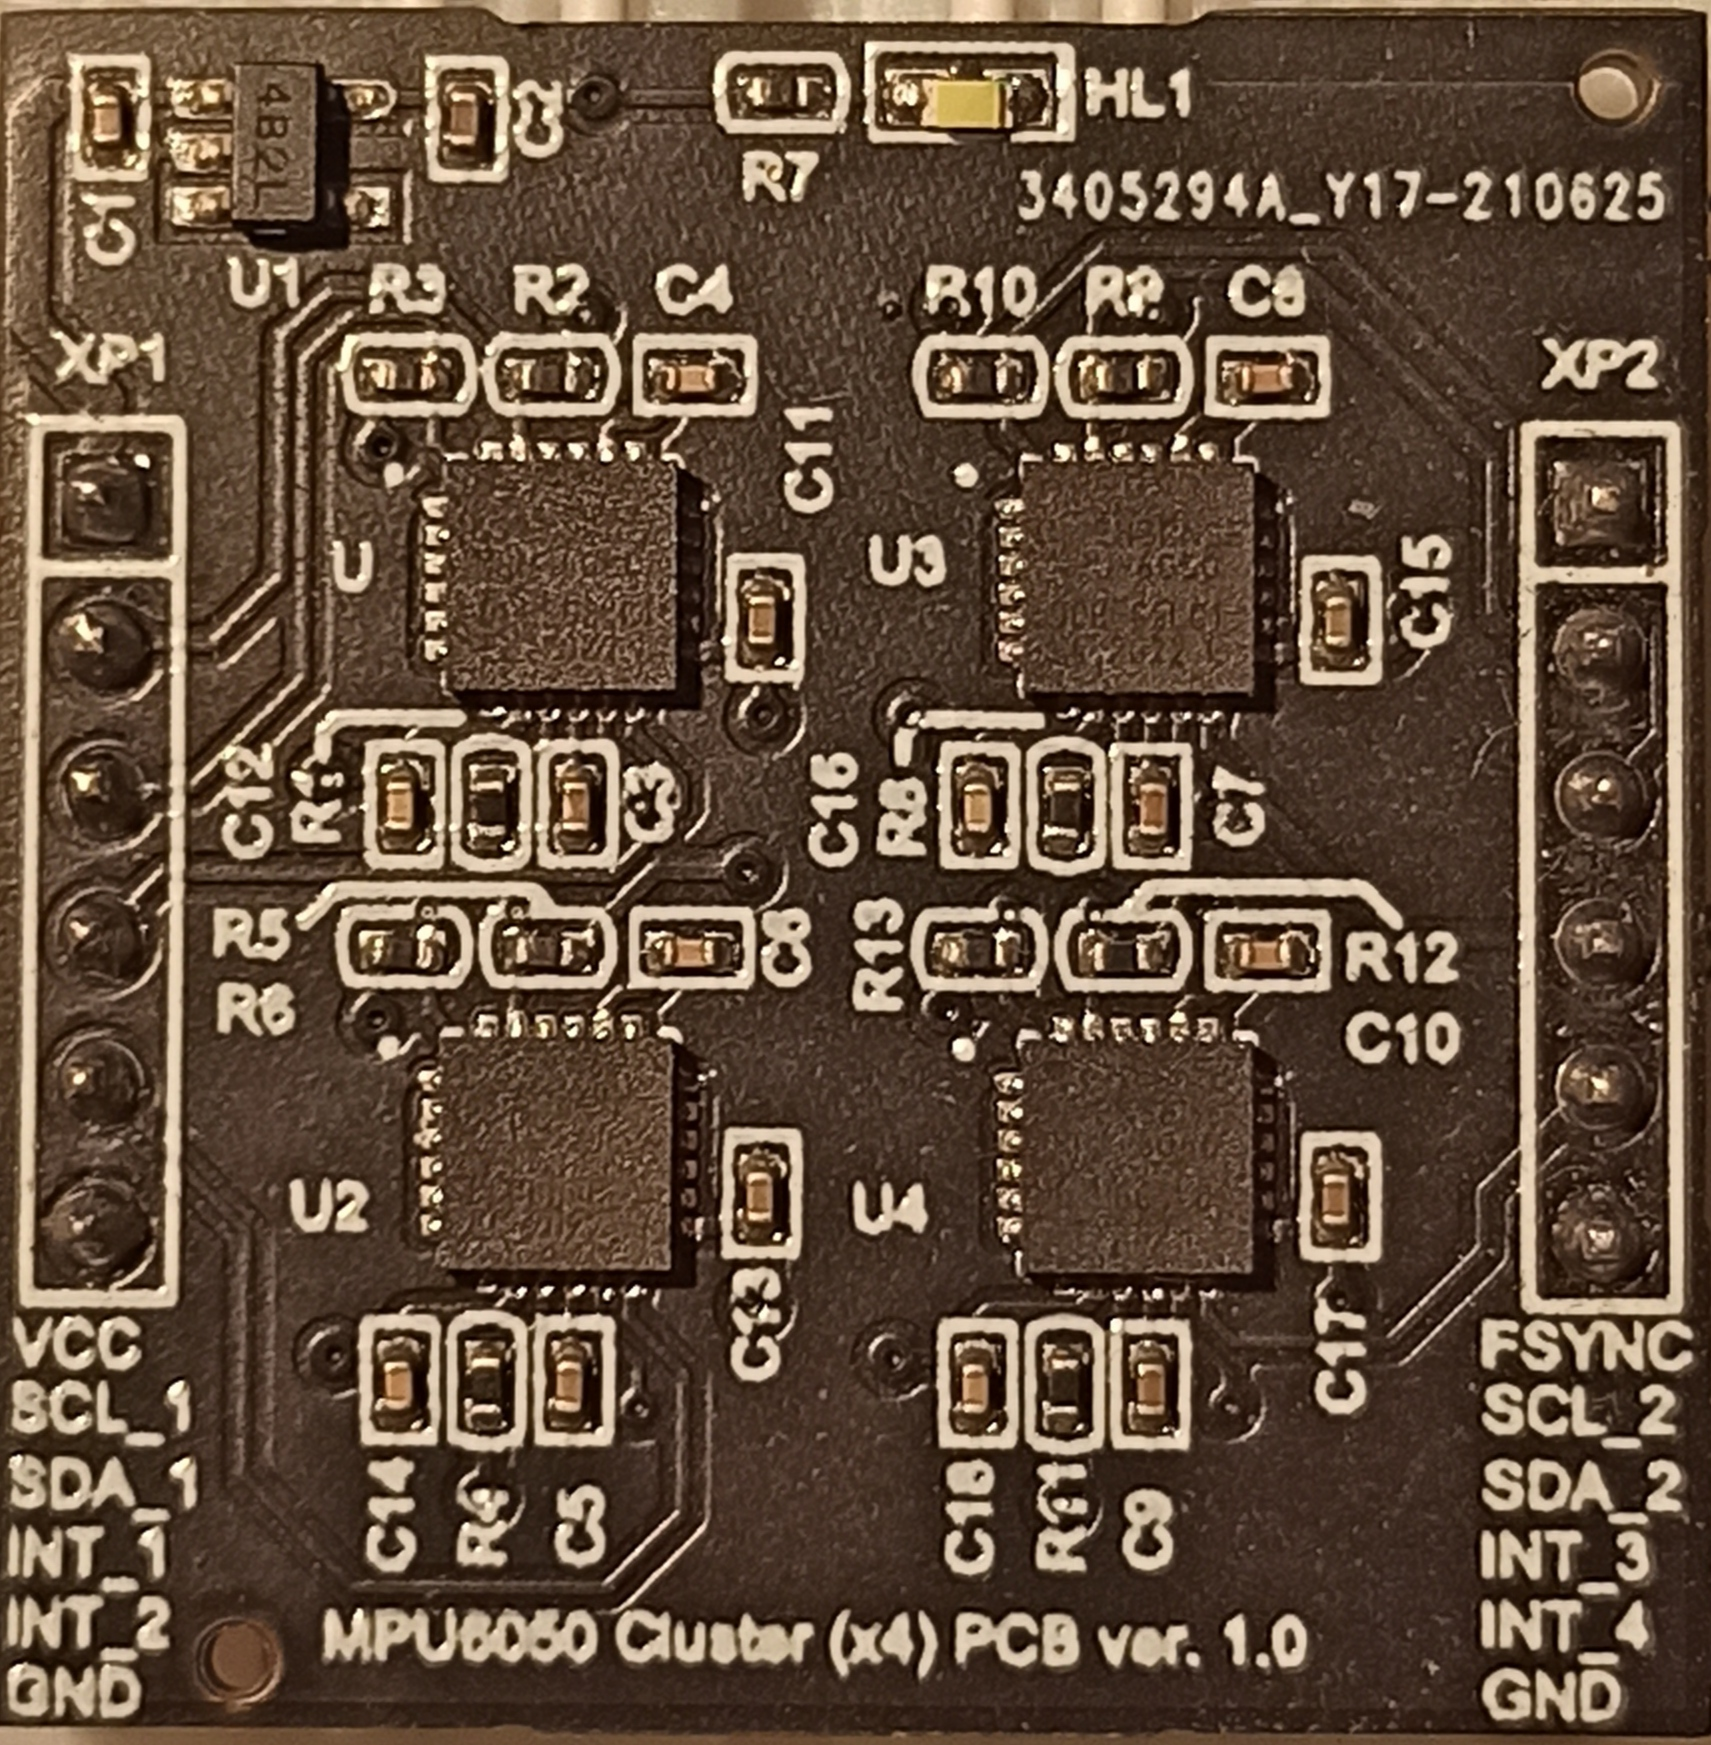
\includegraphics[width=0.4\linewidth]{cluster_pcb.jpg}
	\caption{Печатная плата с кластерным БЧЭ}
	\label{fig:cluster_pcb}
\end{figure}

Для проверки и подтверждения характеристик кластерного бчэ в ходе данной работы была создана печатная плата (Рис. \ref{fig:cluster_pcb}).

В состав разработанного кластерного БЧЭ входят шестиосные датчики фирмы Invensense MPU6050 (трехосный акселерометр и трехосный датчик угловых скоростей).
Данные БЧЭ были выбраны вследствие их наибольшей распространнености и доступности.
Каждый из MPU6050 располагается на печатной плате в вершинах квадрата со стороной 10 мм.
Кроме того, они установлены так, чтобы соответствующие оси чувстительности каждого датчика были параллельны между собой.

Характеристики макетной платы с четырьмя MPU6050. Графики девиации Аллана. Сводная таблица погрешностей IMU.

\section {Оценка выходных погрешностей}

Для оценки точности автономной работы БИНС на базе кластерного блока чувствительных элементов были использованы уравнения ошибок автономной работы ИНС. Данные уравнения учитывают медленно изменяющуюся составляющую ошибки, не зависящую от горизонтального ускорения объекта. Нестационарные погрешности, зависящие от ускорения и обусловленные погрешностью масштабных коэффициентов акселерометров, представляют собой высокочастотную ошибку, модулирующую медленно изменяющуюся шулеровскую, не учитываются в данной модели. 


Для связи выходных параметров ИНС (крен, тангаж, курс, широта, долгота) использованы следующие зависимости:  


\begin{equation}
	\label{eq:phi_x}
	\begin{gathered}
		\varPhi_x(t) = \varPhi_x(0) \cos \nu t - 
		U \cos \phi \frac {\sin \nu t} {\nu} \varPhi_z(0) - 
		\frac{\sin \nu t}{ \nu R} \delta V_y(0) +
		\frac{\sin \nu t}{\nu} \xi_x -\\ 
		U \cos \varPhi \frac{1-\cos \nu t}{\nu^2}\xi_z - 
		\frac{1-\cos \nu t}{\nu^2R} B_y(0)
	\end{gathered}
\end{equation}


\begin{equation}
	\label{eq:phi_y}
		\begin{gathered}
		\varPhi_y(t) = \varPhi_y(0) \cos \nu t + 
		\frac {\sin \nu t} {\nu R} \delta V_x(0) +
		\frac{\sin \nu t}{\nu} \xi_y +\\  
		\frac{1 - \cos \nu t}{ \nu^2 R} B_y(0)
	\end{gathered}
\end{equation}


\begin{equation}
	\label{eq:phi_z}
	\begin{gathered}
		\varPhi_z(t) = \varPhi_x(0) U \cos \phi t + 
		\varPhi_y(0) \tg \phi + \frac{ \tg \phi \sin \nu t }{ \nu R } \delta V_x(0) - \\
		(t - \frac{\sin \nu t}{\nu}) \tg \phi \xi_y + \tg \phi \frac{ 1-\cos \nu t }{ \nu^2 R } B_x(0) + \\
		\varPhi_z(0) + \xi_z t
	\end{gathered}
\end{equation}


\begin{equation}
	\label{eq:V_e}
	\begin{gathered}
		\delta V_e(t) = - \varPhi_y(0) R \sin \nu t + \delta V_x(0) \cos \nu t - \xi_y R (1 - \cos \nu t) + \\
		\frac{\sin \ nu t}{ \nu } B_x(0)
	\end{gathered}
\end{equation}


\begin{equation}
	\label{eq:V_n}
	\begin{gathered}
		\delta V_n(t) = - \varPhi_x(0) R \sin \nu t + \delta V_y(0) \cos \nu t + \xi_x R (1 - \cos \nu t) + \\
		\frac{\sin \ nu t}{ \nu } B_y(0)
	\end{gathered}
\end{equation}

\begin{equation}
	\label{eq:lambda}
	\begin{gathered}
		\lambda (t) = \int \frac{\delta V_e(t)}{R \cos \phi} dt
	\end{gathered}
\end{equation}

\begin{equation}
	\label{eq:phi}
	\begin{gathered}
		\phi (t) = \int \frac{\delta V_n(t)}{R \cos \phi} dt
	\end{gathered}
\end{equation}



\vspace{0.5cm}
где { \large $ \nu = \sqrt{ \frac{g}{R} } $ } - шулеровская частота колебания;


\vspace{0.5cm}
{\large $ B_x(0), B_y(0) $} - смещения нулей акселерометра;


\vspace{0.5cm}
{\large $ \xi_x, \xi_y, \xi_z $} - дрейф гироскопа;


\vspace{0.5cm}
Для оценки остаточной случайной составляющей погрешности акселерометра и гироскопа, с целью использования
данных значений в уравнениях  ~(\ref{eq:phi_x}),~(\ref{eq:phi_y}),~(\ref{eq:phi_z}),~(\ref{eq:V_e}),~(\ref{eq:V_n}), ~(\ref{eq:lambda})~(\ref{eq:phi}) проведена запись показаний чувствиетльных элементов на протяжении 2-ух часов. По результатам измерений построены графики девиации Аллана. 

\newpage

\begin{figure}[h!]
	\centering
	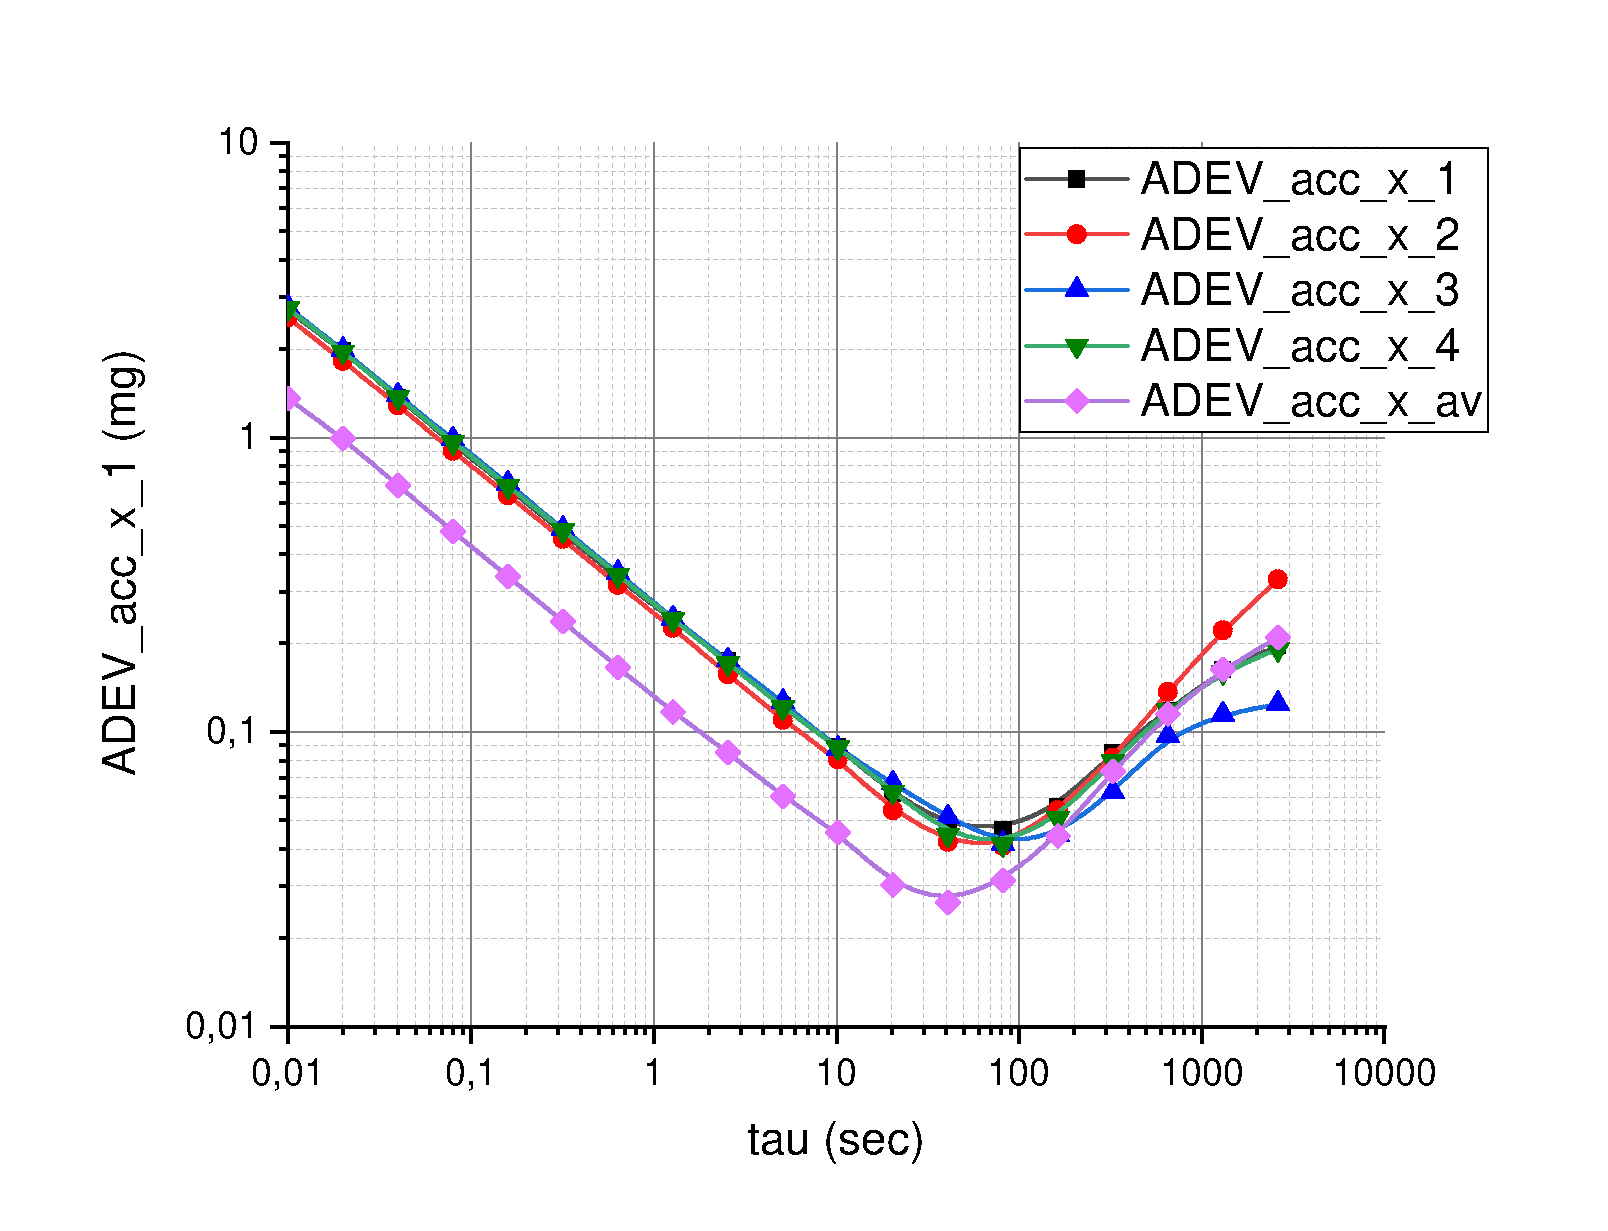
\includegraphics[width=0.9\linewidth]{acc_x_adev.pdf}
	\caption{График девиации Аллана}
	\label{fig:mpr}
\end{figure}


Полученный график Рис.\ref{fig:mpr} девиации Аллана позволяет оценить остаточную случайную погрешность, которая будет присутствовать в выходных данных показаний акселерометров в составе кластерного инерциального измерительного блока. Исходя из уравнений ~(\ref{eq:phi_x}) -- ~(\ref{eq:phi}) остаточная погрешность акселерометра не вносит существенный вклад в ошибку определения выходных координат. Данная ошибка будет влиять исключительно на расчет пространственной ориентации.  


Ниже представлены графики нарастания ошибки определения угла тангажа и крена в течение 5 секунд автономной работы инерциальной навигационной системы. 


\begin{figure}[h]
	\caption{Нарастание ошибки в определении тангажа}
	\label{fig:pitch}
\end{figure}


\begin{figure}[h]
	\caption{Нарастание ошибки в определении крена}
	\label{fig:roll}
\end{figure}

 
Дрейф гироскопов является основной составляющей ошибки определения координат в процессе автономной работы ИНС. Именно поэтому основной задачей исследования точности чувствительных элементов был анализ остаточных погрешностей гироскопов. Из графика (Рис.\ref{fig:mpr}) видно, что значение дрейфа на интервале осреднения 0.01 с. не превышает \SI[per-mode=symbol]{}{\degree\per\second}

\newpage

\begin{figure}[h!]
	\centering
	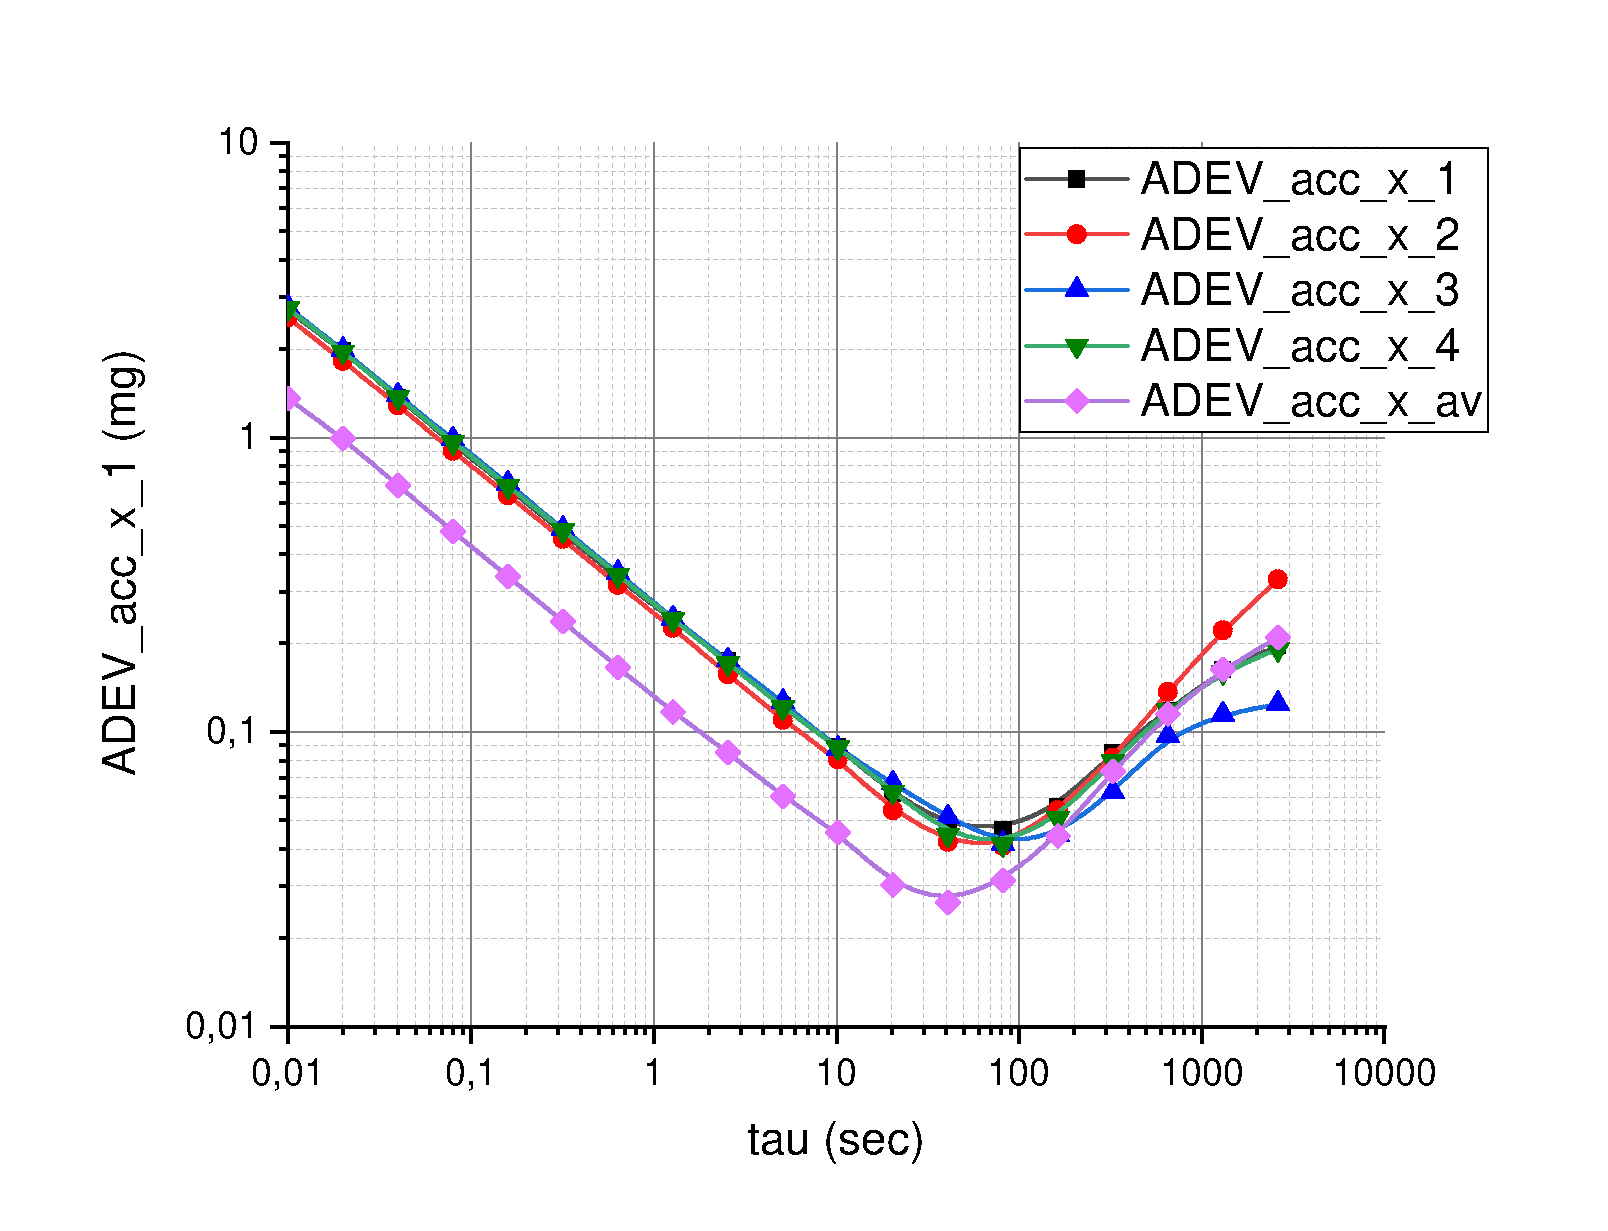
\includegraphics[width=0.9\linewidth]{acc_x_adev.pdf}
	\caption{График девиации Аллана}
	\label{fig:mpr}
\end{figure}


Воспользуемся полученным значением в уравнении ошибок ИНС.

\begin{figure}[h!]
	\caption{График нарастания ошибки в определении широты места}
	\label{fig:lat_error}
\end{figure}


\begin{figure}[h!]
	\caption{График нарастания ошибки в определении долготы места}
	\label{fig:long_error}
\end{figure}

\newpage

\newpage
\section {Интеграция ИНС/ГНСС}

 
 Основной целью интеграции кластерного инерциального блока с навигационным приемником является повышение
 надежности и точности выдаваемого им решения. Для обеспечения максимальной надежности интегрированного алгоритма позиционирования необходимо воспользоваться соответсвующей схемой интеграции двух систем. 
 В данной работе используется OEM плата спутникового навигационного приемника компании NTLab. Данная плата позволяет пользователю получить доступ к срезу кодовых и фазовых измерений на текущую эпоху. Таким образом, тесная схема интеграции ИНС и СНС, которая предполагает использование псевдодальностей СНС и псевдодальности ИНС, видится наиболее оптимальным вариантом. 
 
 Модель системы для расчета углов оринетации, скорости и координат ИНС: 
 
 
 \begin{equation}
 	\label{eq:att_ins}
 	\begin{gathered}
	
 	\end{gathered}
 \end{equation}


\begin{equation}
	\label{eq:vel_ins}
	\begin{gathered}
		
	\end{gathered}
\end{equation}

\begin{equation}
	\label{eq:coord_ins}
	\begin{gathered}
		
	\end{gathered}
\end{equation}
 
 

\section {Сравнение кластера и аналогичного по характеристикам IMU}
Я считаю, что было бы круто сравнить данный кластер со схожим по характеристикам IMU, так как я в abstract писал, что у нас COST-EFFECTIVE решение.

\begin{thebibliography}{00}
	\bibitem{b2} Author1 Article1
\end{thebibliography}


\end {document}